% =====================================================================
%  Cellular Respiration · Student Mission Booklet · Grade 11 AP Biology
%  Al-Hayat International School, Aramoun, Lebanon
%  Compile with XeLaTeX (twice). Needs the Inter font and
%  assets/his-logo.png. Minimum font size: 12 pt.
%  Question numbers match the board pages (Q1.1 … Q6.6).
% =====================================================================
\documentclass[12pt,a4paper]{article}
\usepackage[a4paper,top=1.5cm,bottom=1.6cm,left=1.6cm,right=1.6cm,headheight=32pt,headsep=10pt]{geometry}
\usepackage{fontspec}
\setmainfont{Inter}[BoldFont={Inter SemiBold}]
\newfontfamily\display{Inter Display}[BoldFont={Inter Display Bold}]
\usepackage{amsmath}
\usepackage[table]{xcolor}
\usepackage{graphicx,tikz,enumitem,array,tabularx,fancyhdr,lastpage,needspace,multicol}
\usepackage[most]{tcolorbox}
\usetikzlibrary{arrows.meta,positioning,calc,shapes.geometric,decorations.pathmorphing}
\graphicspath{{assets/}}

% ---------- colours (HIS logo + the board pages' molecule colours) ----------
\definecolor{navy}{HTML}{0A4F8F}\definecolor{hisblue}{HTML}{0068B0}\definecolor{hissky}{HTML}{00B0E0}
\definecolor{hisgold}{HTML}{F8D000}\definecolor{hisred}{HTML}{F2361C}\definecolor{muted}{HTML}{4E6176}
\definecolor{good}{HTML}{1D8A4A}\definecolor{goodsoft}{HTML}{E3F3E7}
\definecolor{rose}{HTML}{D8321A}\definecolor{rosesoft}{HTML}{FDEAE6}
\definecolor{goldsoft}{HTML}{FFF6CF}\definecolor{golddark}{HTML}{8A6D00}
\definecolor{cglu}{HTML}{2E8B47}\definecolor{cpyr}{HTML}{E08A00}\definecolor{catp}{HTML}{F2361C}\definecolor{cadp}{HTML}{E25B2B}
\definecolor{cnadh}{HTML}{6A3FC0}\definecolor{cnad}{HTML}{8A63D2}\definecolor{cfad}{HTML}{C2378F}\definecolor{cco}{HTML}{5B6B7C}
\definecolor{co}{HTML}{1F9E97}\definecolor{cwat}{HTML}{0FA3D8}\definecolor{clac}{HTML}{B5452B}\definecolor{ceth}{HTML}{7A8B00}
\definecolor{outer}{HTML}{F29A55}\definecolor{inner}{HTML}{E0612A}\definecolor{mtxc}{HTML}{FFE4C7}\definecolor{ims}{HTML}{FFF3C4}
\definecolor{cyto}{HTML}{E8EEF6}
\definecolor{sgly}{HTML}{2E8B47}\definecolor{skre}{HTML}{E08A00}\definecolor{setc}{HTML}{C2410C}\definecolor{sfer}{HTML}{8A63D2}\definecolor{ssho}{HTML}{0068B0}\definecolor{spow}{HTML}{F2361C}

\setlength{\parindent}{0pt}\setlength{\parskip}{4pt}\linespread{1.08}
\setlist{itemsep=1pt,topsep=2pt}
\setlength{\columnsep}{18pt}

% ---------- header / footer ----------
\pagestyle{fancy}\fancyhf{}
\renewcommand{\headrule}{\hbox to\headwidth{\color{hisred}\leaders\hrule height 1.4pt\hskip0.25\headwidth\color{hisgold}\leaders\hrule height 1.4pt\hskip0.25\headwidth\color{hissky}\leaders\hrule height 1.4pt\hskip0.25\headwidth\color{hisblue}\leaders\hrule height 1.4pt\hfill}}
\fancyhead[L]{\raisebox{-0.32\height}{
\includegraphics[height=0.9cm]{his-logo.png}}\hspace{6pt}\color{navy}\textbf{Al-Hayat International School}}
\fancyhead[R]{\color{muted}Grade 11 AP Biology · Cellular Respiration}
\fancyfoot[C]{\color{muted}Page \thepage\ of \pageref{LastPage}}
\fancypagestyle{first}{\fancyhf{}\renewcommand{\headrule}{}\fancyfoot[C]{\color{muted}Page \thepage\ of \pageref{LastPage}}}

% ---------- building blocks ----------
\newcommand{\mission}[3]{\par\needspace{14\baselineskip}\vspace{3pt}\noindent\begin{tikzpicture}
  \node[fill=#1,text=white,rounded corners=9pt,inner sep=6pt,font=\bfseries] (b) {#2};
  \node[right=8pt of b,font=\display\bfseries\LARGE,text=navy] {#3};\end{tikzpicture}\par\vspace{-2pt}}
\newcommand{\sect}[1]{\par\needspace{6\baselineskip}\vspace{2pt}{\display\bfseries\large\color{navy}#1}\par}
\newcommand{\Q}[1]{\textbf{\color{hisblue}#1}\ }
\newcommand{\blank}[1][3cm]{\rule[-2pt]{#1}{0.6pt}}
\newcommand{\lines}[1]{\par\vspace{-2pt}\begin{tikzpicture}
  \foreach \i in {1,...,#1}{\draw[muted!45] (0,-\i*0.86) -- (\linewidth-0.4pt,-\i*0.86);}
  \path (0,0) (0,-#1*0.86-0.1);\end{tikzpicture}\par}
\newcommand{\cb}{\tikz[baseline=-3pt]\draw[muted,line width=0.8pt,rounded corners=1.5pt] (0,-0.17) rectangle (0.38,0.21);}
\newcommand{\numbox}{\tikz[baseline=-4pt]\draw[muted,line width=0.9pt,rounded corners=2pt] (0,-0.25) rectangle (0.75,0.32);}
\newcommand{\bx}[1][1.6cm]{\tikz[baseline=-4pt]\draw[muted,line width=0.9pt,rounded corners=2pt] (0,-0.28) rectangle (#1,0.36);}
\newcommand{\m}[2]{\textcolor{#1}{\textbf{#2}}}
\newcommand{\move}{\textcolor{golddark}{\textbf{Move!}}\ }

\tcbset{base/.style={enhanced,boxrule=0pt,leftrule=5pt,arc=6pt,left=9pt,right=9pt,top=4pt,bottom=4pt,
        fonttitle=\bfseries,coltitle=#1,attach title to upper={\ }}}
\newtcolorbox{hook}[1][]{base=golddark,colback=goldsoft,colframe=hisgold!90!black,title={#1}}
\newtcolorbox{teaser}[1][]{base=rose,colback=rosesoft,colframe=rose,title={#1}}
\newtcolorbox{real}[1][]{base=good,colback=goodsoft,colframe=good,title={#1}}

\tikzset{tok/.style={rounded corners=7pt,text=white,font=\bfseries,inner xsep=6pt,inner ysep=3pt},
  arr/.style={-{Latex[length=3mm]},line width=1.5pt}}
\renewcommand{\arraystretch}{1.25}
\newcolumntype{C}[1]{>{\centering\arraybackslash}p{#1}}

\begin{document}
\thispagestyle{first}

% ===================== TITLE =====================
\begin{tcolorbox}[enhanced,colback=navy,colframe=navy,arc=10pt,left=12pt,right=12pt,top=9pt,bottom=9pt,
  interior style={left color=navy!90!black,right color=hissky}]
\color{white}
\begin{tabular}{@{}m{2.9cm}@{}m{13.6cm}@{}}
\tikz\node[fill=white,rounded corners=8pt,inner sep=4pt]{
\includegraphics[height=2.2cm]{his-logo.png}}; &
{\bfseries\large Al-Hayat International School}\newline Aramoun, Mount Lebanon · American High School Program\par\vspace{5pt}
{\display\bfseries\fontsize{23}{27}\selectfont Mission: Power the Cell}\par\vspace{1pt}
Cellular Respiration · Grade 11 AP Biology · Student Mission Booklet\\
\end{tabular}
\end{tcolorbox}
\vspace{-8pt}\noindent\tikz{\foreach \c [count=\i from 0] in {hisred,hisgold,hissky,hisblue}{\fill[\c] (\i*0.25*\linewidth,0) rectangle ++(0.25*\linewidth,0.14);}}\par
\begin{tabularx}{\linewidth}{@{}l X l p{2.4cm} l p{3.2cm}@{}}
\textbf{Name:} & \hrulefill & \textbf{Section:} & \hrulefill & \textbf{Team:} & \hrulefill
\end{tabularx}

\begin{hook}[The story.]
Lara is running the \textbf{Beirut Marathon}: 42 km. Every step costs her muscles energy as \m{catp}{ATP}. Over six missions you will follow one \m{cglu}{glucose} molecule from her breakfast man'oushe all the way to ATP. Question numbers match the board.
\end{hook}

% ===================== MISSION 1 =====================
\mission{spow}{Mission 1}{The Powerhouse}
\Q{Q1.1 Gut feeling.} How does the food Lara eats become energy for her muscles?
\lines{1}
\Q{Q1.2} \move After the 30-second jog, name two things that changed in your body. Why?
\lines{2}
\Q{Q1.3} Complete the equation for aerobic respiration.
\[\text{C}_6\text{H}_{12}\text{O}_6\;+\;\underline{\hspace{2.2cm}}\ \xrightarrow{\text{\normalsize enzymes}}\ \underline{\hspace{2.2cm}}\;+\;\underline{\hspace{2.2cm}}\;+\;\underline{\hspace{2.4cm}}\]
\begin{teaser}[Q1.4 Brain teaser:]
Compare this equation with the photosynthesis equation. What do you notice?
\lines{1}
\end{teaser}

\sect{Inside the mitochondrion}
\begin{minipage}[c]{0.6\linewidth}
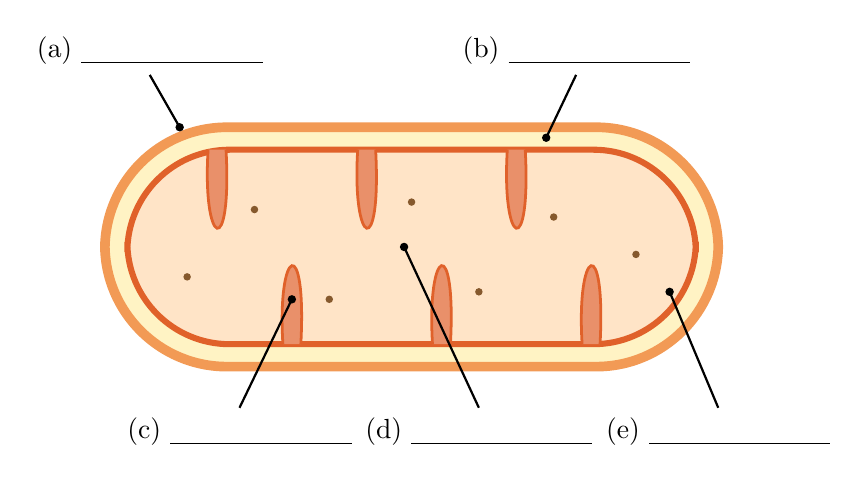
\begin{tikzpicture}[scale=0.95]
  \filldraw[fill=ims,draw=outer,line width=3.5pt,rounded corners=1.55cm] (0,0) rectangle (8.2,3.2);
  \filldraw[fill=mtxc,draw=inner,line width=2.2pt,rounded corners=1.3cm] (0.3,0.3) rectangle (7.9,2.9);
  \foreach \x/\u in {1.5/1,2.5/0,3.5/1,4.5/0,5.5/1,6.5/0}{
    \ifnum\u=1 \filldraw[fill=inner!70,draw=inner,line width=1pt] (\x-0.12,2.9) .. controls (\x-0.2,1.6) and (\x+0.2,1.4) .. (\x+0.12,2.9);
    \else \filldraw[fill=inner!70,draw=inner,line width=1pt] (\x-0.12,0.3) .. controls (\x-0.2,1.6) and (\x+0.2,1.8) .. (\x+0.12,0.3); \fi}
  \foreach \p in {(1.1,1.2),(2.0,2.1),(3.0,0.9),(4.1,2.2),(5.0,1.0),(6.0,2.0),(7.1,1.5)}{\fill[brown!70!black] \p circle (0.05);}
  % leaders
  \draw[line width=0.8pt] (1.0,3.2) -- (0.6,3.9) node[above,font=\normalsize] {(a) \blank[2.3cm]};
  \draw[line width=0.8pt] (5.9,3.06) -- (6.3,3.9) node[above,font=\normalsize] {(b) \blank[2.3cm]};
  \draw[line width=0.8pt] (2.5,0.9) -- (1.8,-0.55) node[below,font=\normalsize] {(c) \blank[2.3cm]};
  \draw[line width=0.8pt] (4.0,1.6) -- (5.0,-0.55) node[below,font=\normalsize] {(d) \blank[2.3cm]};
  \draw[line width=0.8pt] (7.55,1.0) -- (8.2,-0.55) node[below,font=\normalsize] {(e) \blank[2.3cm]};
  \fill (1.0,3.2) circle (1.6pt) (5.9,3.06) circle (1.6pt) (2.5,0.9) circle (1.6pt) (4.0,1.6) circle (1.6pt) (7.55,1.0) circle (1.6pt);
\end{tikzpicture}
\end{minipage}\hfill
\begin{minipage}[c]{0.37\linewidth}\raggedright
\Q{Q1.5} Label the parts: \textbf{outer membrane, intermembrane space, inner membrane, cristae, matrix}.\par\vspace{4pt}
\textit{Hint: (b) is the narrow gap; (e) is the inner membrane at the end of the mitochondrion.}
\end{minipage}

\needspace{7\baselineskip}\begin{multicols}{2}
\begin{teaser}[Q1.6 Brain teaser:]
Why is the inner membrane folded into cristae?
\lines{2}
\end{teaser}
\columnbreak
\begin{real}[Q1.7 Real world:]
Why do heart and leg muscles have so many mitochondria?
\lines{2}
\end{real}
\end{multicols}

\Q{Q1.8} What is the difference between ATP and ADP?
\lines{2}
\begin{teaser}[Q1.9 Brain teaser:]
You hold only about 250 g of ATP, yet use about your own body mass in ATP every day. How?
\lines{1}
\end{teaser}
\Q{Q1.10} Write where each stage happens.\quad
\begin{tabular}{@{}lp{6.2cm}@{}}
Glycolysis & \hrulefill\\ Krebs cycle & \hrulefill\\ Electron transport chain & \hrulefill
\end{tabular}

% ===================== MISSION 2 =====================
\mission{sgly}{Mission 2}{Glycolysis: splitting sugar}
\begin{center}
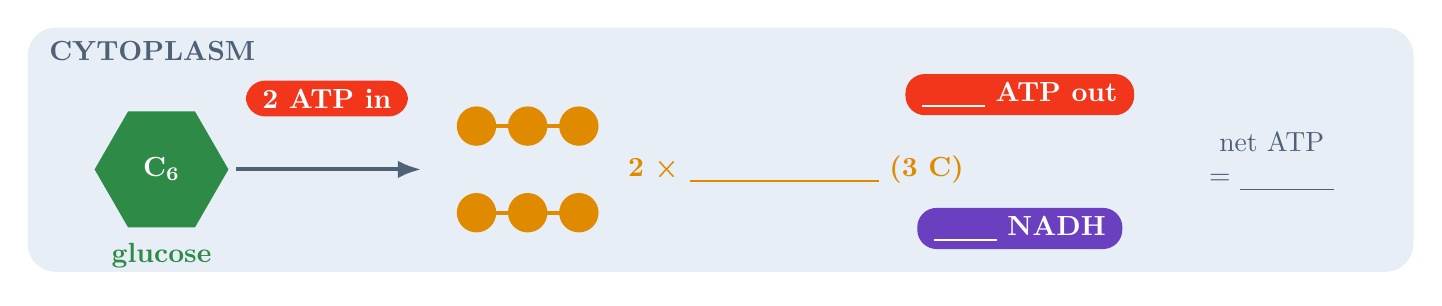
\begin{tikzpicture}[x=1cm,y=1cm]
  \fill[cyto,rounded corners=10pt] (0,0) rectangle (17.6,3.1);
  \node[anchor=north west,text=muted,font=\bfseries] at (0.15,3.05) {CYTOPLASM};
  \node[regular polygon,regular polygon sides=6,fill=cglu,minimum size=1.7cm,text=white,font=\bfseries] (g) at (1.7,1.3) {C\textsubscript{6}};
  \node[text=cglu,font=\bfseries] at (1.7,0.2) {glucose};
  \draw[arr,muted] (2.65,1.3) -- (5.0,1.3);
  \node[tok,fill=catp] at (3.8,2.2) {2 ATP in};
  \foreach \y in {1.85,0.75}{\foreach \i in {0,1,2}{\fill[cpyr] (5.7+\i*0.65,\y) circle (0.25);}\draw[cpyr,line width=1.5pt] (5.7,\y) -- (7.0,\y);}
  \node[text=cpyr,font=\bfseries,anchor=west] at (7.5,1.3) {2 × \blank[2.4cm]\ (3 C)};
  \node[tok,fill=catp] at (12.6,2.25) {\blank[0.8cm] ATP out};
  \node[tok,fill=cnadh] at (12.6,0.55) {\blank[0.8cm] NADH};
  \node[text=muted,align=center,font=\normalsize] at (15.8,1.4) {net ATP\\= \blank[1.2cm]};
\end{tikzpicture}
\end{center}
\Q{Q2.1} Glycolysis happens in the \blank[3.6cm]. Does it need oxygen? \blank[2cm]

\Q{Q2.2} Number the steps 1–5 in order.\\[2pt]
\begin{tabularx}{\linewidth}{@{}p{1.1cm}X@{}}
\numbox & The glucose is split into two 3-carbon halves.\\
\numbox & The 2 pyruvates move into the mitochondrion (if oxygen is present).\\
\numbox & Glucose (6 carbons) enters the cytoplasm.\\
\numbox & 4 ATP and 2 NADH are made; each half becomes pyruvate.\\
\numbox & 2 ATP are spent to activate the glucose.\\
\end{tabularx}

\Q{Q2.3} Complete:\quad \underline{\hspace{2.6cm}} $\xrightarrow{\text{\normalsize cytoplasm}}$ 2\,\underline{\hspace{2.6cm}} + 2\,\underline{\hspace{1.8cm}} (net) + 2\,\underline{\hspace{1.8cm}}

\needspace{7\baselineskip}\begin{multicols}{2}
\begin{teaser}[Q2.4 Brain teaser:]
Spend 2 ATP, earn 4 ATP. Net gain? \blank[1.5cm]
\end{teaser}
\columnbreak
\Q{Q2.5} Each pyruvate has \blank[1cm] carbons. Is any carbon lost? \blank[1.6cm]
\end{multicols}

\Q{Q2.6} Tick one box for each molecule in glycolysis.
\begin{center}
\begin{tabular}{|l|*{8}{C{1.55cm}|}}
\hline\rowcolor{goodsoft}
 & \bfseries glucose & \bfseries 2 ATP spent & \bfseries 2 NAD⁺ & \bfseries 2 pyruvate & \bfseries 4 ATP made & \bfseries 2 NADH & \bfseries oxygen & \bfseries CO\textsubscript{2}\\\hline
\textbf{Input} & \cb&\cb&\cb&\cb&\cb&\cb&\cb&\cb\\\hline
\textbf{Output} & \cb&\cb&\cb&\cb&\cb&\cb&\cb&\cb\\\hline
\textbf{Not part} & \cb&\cb&\cb&\cb&\cb&\cb&\cb&\cb\\\hline
\end{tabular}
\end{center}
\needspace{7\baselineskip}\begin{multicols}{2}
\begin{teaser}[Q2.7 Brain teaser:]
Almost every living thing does glycolysis, without oxygen. What does this suggest?
\lines{2}
\end{teaser}
\columnbreak
\begin{real}[Q2.8 Real world:]
Why can't Lara run a marathon using glycolysis alone?
\lines{2}
\end{real}
\end{multicols}

% ===================== MISSION 3 =====================
\mission{skre}{Mission 3}{The Krebs cycle}
\begin{minipage}[c]{0.44\linewidth}
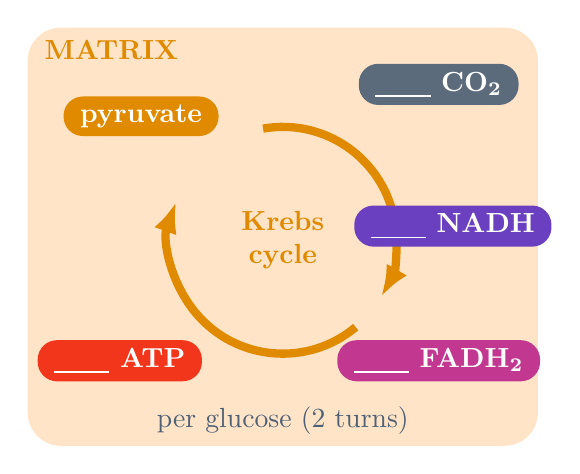
\begin{tikzpicture}[scale=0.9]
  \fill[mtxc,rounded corners=12pt] (-3.6,-2.9) rectangle (3.6,3.0);
  \node[anchor=north west,text=skre,font=\bfseries] at (-3.5,2.95) {MATRIX};
  \draw[skre,line width=3pt,-{Latex[length=4mm]}] (100:1.6) arc (100:-30:1.6);
  \draw[skre,line width=3pt,-{Latex[length=4mm]}] (-50:1.6) arc (-50:-200:1.6);
  \node[text=skre,font=\bfseries,align=center] at (0,0) {Krebs\\cycle};
  \node[tok,fill=cpyr] at (-2.0,1.75) {pyruvate};
  \node[tok,fill=cco] at (2.2,2.2) {\blank[0.7cm] CO\textsubscript{2}};
  \node[tok,fill=cnadh] at (2.4,0.2) {\blank[0.7cm] NADH};
  \node[tok,fill=cfad] at (2.2,-1.7) {\blank[0.7cm] FADH\textsubscript{2}};
  \node[tok,fill=catp] at (-2.3,-1.7) {\blank[0.7cm] ATP};
  \node[text=muted,font=\normalsize] at (0,-2.55) {per glucose (2 turns)};
\end{tikzpicture}
\end{minipage}\hfill
\begin{minipage}[c]{0.53\linewidth}\raggedright
\Q{Q3.1} The Krebs cycle happens in the \blank[3cm].\par\vspace{4pt}
\Q{Q3.2} What happens to pyruvate in the link step?
\lines{2}
\begin{teaser}[Q3.3 Brain teaser:]
How many turns per glucose? Why? \lines{1}
\end{teaser}
\Q{Q3.4} Fill in the totals on the diagram (per glucose).
\end{minipage}

\Q{Q3.5} Tick one box for each molecule in the link step + Krebs cycle.
\begin{center}
\begin{tabular}{|l|*{8}{C{1.55cm}|}}
\hline\rowcolor{goldsoft}
 & \bfseries pyruvate & \bfseries NAD⁺ & \bfseries FAD & \bfseries ADP & \bfseries CO\textsubscript{2} & \bfseries NADH & \bfseries FADH\textsubscript{2} & \bfseries ATP\\\hline
\textbf{Input} & \cb&\cb&\cb&\cb&\cb&\cb&\cb&\cb\\\hline
\textbf{Output} & \cb&\cb&\cb&\cb&\cb&\cb&\cb&\cb\\\hline
\end{tabular}
\end{center}
\begin{teaser}[Q3.6 Brain teaser:]
The Krebs cycle never uses oxygen itself, yet it stops if oxygen runs out. Why?
\lines{2}
\end{teaser}
\Q{Q3.7} \move The limewater test. Prediction: which turns limewater milky faster, air breathed in or breathed out?
\blank[6cm]\par\vspace{3pt}
\begin{tabular}{|l|C{3.6cm}|C{3.6cm}|}
\hline\rowcolor{cyto} & \textbf{Room air pumped in} & \textbf{Air breathed out}\\\hline
Presses to turn milky & & \\\hline
\end{tabular}\par
Explain using the Krebs cycle:
\lines{2}
\begin{real}[Q3.8 Real world:]
When a person loses 10 kg of fat, where does most of the mass go?
\lines{1}
\end{real}

% ===================== MISSION 4 =====================
\mission{setc}{Mission 4}{The electron transport chain}
\begin{center}
\begin{tikzpicture}[x=1cm,y=1cm]
  \fill[ims] (0,2.0) rectangle (17.6,3.4); \fill[mtxc] (0,-1.4) rectangle (17.6,0.6);
  \fill[outer!60] (0,0.6) rectangle (17.6,2.0);
  \node[anchor=north west,font=\bfseries,text=golddark] at (0.1,3.4) {INTERMEMBRANE SPACE (high H\textsuperscript{+})};
  \node[anchor=south west,font=\bfseries,text=skre] at (0.1,-1.4) {MATRIX};
  \foreach \x/\c in {3.0/cnad,6.4/co,9.8/hisblue}{\filldraw[fill=\c!80,draw=\c!60!black,rounded corners=10pt] (\x-0.75,0.15) rectangle (\x+0.75,2.45);}
  \node[white,font=\bfseries] at (3.0,1.3) {1}; \node[white,font=\bfseries] at (6.4,1.3) {2}; \node[white,font=\bfseries] at (9.8,1.3) {3};
  \filldraw[fill=gray!40,draw=gray!70!black] (13.2,0.7) rectangle (14.4,1.9); \draw[line width=3pt,gray!70!black] (13.8,0.7) -- (13.8,-0.3); \filldraw[fill=gray!30,draw=gray!70!black] (13.8,-0.65) ellipse (0.9 and 0.45);
  \draw[arr,hisgold!80!black,decorate,decoration={snake,amplitude=1.2pt,segment length=8pt,post length=4pt}] (3.7,1.3) -- (5.6,1.3);
  \draw[arr,hisgold!80!black,decorate,decoration={snake,amplitude=1.2pt,segment length=8pt,post length=4pt}] (7.1,1.3) -- (9.0,1.3);
  \draw[arr,hisgold!80!black] (9.8,0.1) -- (9.8,-0.75);
  \foreach \x in {3.0,6.4,9.8}{\draw[arr,hissky] (\x+0.35,-0.5) -- (\x+0.35,2.95);}
  \draw[arr,hissky,line width=2pt] (13.8,3.1) -- (13.8,2.0);
  \node[tok,fill=cnadh] at (1.0,-0.45) {NADH};
  \node[tok,fill=co] at (8.6,-0.95) {O\textsubscript{2}};
  \node[font=\normalsize,anchor=west] at (10.3,-0.95) {→ \blank[1.6cm]};
  \node[tok,fill=catp] at (16.0,-0.6) {ATP};
  \node[font=\normalsize\bfseries] at (13.8,2.75) {(f) \blank[2.5cm]};
  \node[font=\normalsize,text=hissky!70!black] at (5.0,2.85) {H\textsuperscript{+}};
  \node[font=\normalsize,text=golddark] at (4.7,1.75) {e\textsuperscript{−}};
\end{tikzpicture}
\end{center}
\Q{Q4.1} The electron transport chain is in the \blank[5.2cm]. Label (f) and the product made from O\textsubscript{2}.

\Q{Q4.2} Number the steps 1–5 in order.\\[2pt]
\begin{tabularx}{\linewidth}{@{}p{1.1cm}X@{}}
\numbox & H\textsuperscript{+} flow back through ATP synthase, which makes ATP.\\
\numbox & NADH and FADH\textsubscript{2} drop off their electrons.\\
\numbox & Oxygen catches the electrons and forms water.\\
\numbox & Electrons are passed from protein to protein.\\
\numbox & Their energy pumps H\textsuperscript{+} into the intermembrane space.\\
\end{tabularx}
\begin{teaser}[Q4.3 Brain teaser: the Qaraoun dam.]
In the mitochondrion, what plays the part of the\quad dam \blank[2.8cm]\quad water \blank[2.6cm]\quad turbine \blank[2.8cm]?
\end{teaser}
\Q{Q4.4} What is the job of oxygen in the chain, and what does it become?
\lines{2}
\needspace{6\baselineskip}\Q{Q4.5} Tick one box for each molecule in the electron transport chain.
\begin{center}
\begin{tabular}{|l|*{8}{C{1.55cm}|}}
\hline\rowcolor{rosesoft}
 & \bfseries NADH & \bfseries FADH\textsubscript{2} & \bfseries oxygen & \bfseries ADP & \bfseries ATP & \bfseries water & \bfseries NAD⁺ & \bfseries FAD\\\hline
\textbf{Input} & \cb&\cb&\cb&\cb&\cb&\cb&\cb&\cb\\\hline
\textbf{Output} & \cb&\cb&\cb&\cb&\cb&\cb&\cb&\cb\\\hline
\end{tabular}
\end{center}
\Q{Q4.6} Effect of oxygen: describe and explain what happens to ATP production at 100\%, 50\% and 0\% oxygen.
\lines{3}
\needspace{7\baselineskip}\begin{multicols}{2}
\begin{real}[Q4.7 Real world:]
Why is cyanide deadly within minutes?
\lines{2}
\end{real}
\columnbreak
\begin{real}[Q4.8 Real world:]
Why do climbers feel weak on Everest?
\lines{2}
\end{real}
\end{multicols}
\begin{teaser}[Q4.9 The ATP bill:]
glycolysis \bx[1.1cm] + Krebs \bx[1.1cm] + ETC \bx[1.1cm] = \bx[1.4cm] ATP per glucose
\end{teaser}

% ===================== MISSION 5 =====================
\mission{sfer}{Mission 5}{Fermentation: Plan B}
\Q{Q5.1} \move Breaths per 30 seconds.\par\vspace{2pt}
\begin{center}
\begin{tabular}{|l|C{2.5cm}|C{2.5cm}|C{2.5cm}|C{2.5cm}|}
\hline\rowcolor{cyto} & \textbf{Team 1} & \textbf{Team 2} & \textbf{Team 3} & \textbf{Team 4}\\\hline
At rest & & & & \\\hline
After exercise & & & & \\\hline
Increase & & & & \\\hline
\end{tabular}
\end{center}
\Q{Q5.2} Explain why breathing rate rises during exercise.
\lines{2}
\Q{Q5.3} Lactic acid fermentation:\quad \underline{\hspace{2.4cm}} + NADH $\xrightarrow{\text{\normalsize no O\textsubscript{2}}}$ \underline{\hspace{2.6cm}} + \underline{\hspace{1.8cm}}
\begin{teaser}[Q5.4 Brain teaser:]
Turning pyruvate into lactic acid makes no ATP. So why do muscles bother?
\lines{2}
\end{teaser}
\begin{real}[Q5.5 Real world:]
Why do Lara's legs burn in the sprint, and why does she breathe hard after the finish?
\lines{2}
\end{real}
\Q{Q5.6} Alcoholic fermentation (yeast):\quad pyruvate $\xrightarrow{\text{\normalsize no O\textsubscript{2}}}$ \underline{\hspace{2.6cm}} + \underline{\hspace{3cm}}

\Q{Q5.7} \move The balloon race.\par\vspace{2pt}
\begin{center}
\begin{tabular}{|l|C{2.5cm}|C{2.5cm}|C{2.5cm}|C{2.5cm}|}
\hline\rowcolor{cyto} & \textbf{Team 1} & \textbf{Team 2} & \textbf{Team 3} & \textbf{Team 4}\\\hline
Temperature (°C) & & & & \\\hline
Balloon rank (1 = biggest) & & & & \\\hline
\end{tabular}
\end{center}
Best temperature, and why the hottest flasks failed:
\lines{2}
\begin{real}[Q5.8 Real world:]
Explain why man'oushe dough rises, and how labneh is made.
\lines{2}
\end{real}
\Q{Q5.9} Tick the correct column.
\begin{center}
\begin{tabular}{|l|C{2.6cm}|C{2.6cm}|C{1.6cm}|}
\hline\rowcolor{goodsoft} & \textbf{Lactic acid} & \textbf{Alcoholic} & \textbf{Both}\\\hline
makes lactic acid & \cb & \cb & \cb \\\hline
makes ethanol & \cb & \cb & \cb \\\hline
releases CO\textsubscript{2} & \cb & \cb & \cb \\\hline
happens in human muscle cells & \cb & \cb & \cb \\\hline
happens in yeast & \cb & \cb & \cb \\\hline
recycles NAD⁺ & \cb & \cb & \cb \\\hline
2 ATP per glucose & \cb & \cb & \cb \\\hline
no oxygen needed & \cb & \cb & \cb \\\hline
\end{tabular}
\end{center}
\Q{Q5.10} Aerobic respiration releases \blank[1.2cm] ATP; fermentation \blank[1.2cm]. That is \blank[1.2cm] times more because
\lines{1}

% ===================== MISSION 6 =====================
\mission{ssho}{Mission 6}{The Showdown}
\needspace{7\baselineskip}\begin{multicols}{2}
\Q{Q6.1} What does the chloroplast pass to the mitochondrion, and what comes back?
\lines{3}
\columnbreak
\begin{teaser}[Q6.2 Brain teaser:]
Sunlight off: which organelle stops first? Can the other keep going forever?
\lines{2}
\end{teaser}
\end{multicols}
\begin{minipage}[t]{0.5\linewidth}
\Q{Q6.3} Photosynthesis (P), respiration (R) or both (B)?\par\vspace{2pt}
\renewcommand{\arraystretch}{1.18}
\begin{tabular}{@{}l c@{}}
happens in chloroplasts & \bx[0.9cm]\\
happens in mitochondria & \bx[0.9cm]\\
uses carbon dioxide & \bx[0.9cm]\\
releases carbon dioxide & \bx[0.9cm]\\
uses oxygen & \bx[0.9cm]\\
releases oxygen & \bx[0.9cm]\\
stores energy in glucose & \bx[0.9cm]\\
releases energy from glucose & \bx[0.9cm]\\
happens in plant cells & \bx[0.9cm]\\
makes ATP & \bx[0.9cm]\\
\end{tabular}
\end{minipage}\hfill
\begin{minipage}[t]{0.48\linewidth}
\Q{Q6.4} \move Stage race: write G (glycolysis), K (link + Krebs), E (ETC) or F (fermentation).\par\vspace{2pt}
\renewcommand{\arraystretch}{1.18}
\begin{tabular}{@{}l c@{}}
splits glucose & \bx[0.8cm]\\
spends 2 ATP to start & \bx[0.8cm]\\
happens in the matrix & \bx[0.8cm]\\
acetyl joins a 4-C molecule & \bx[0.8cm]\\
makes FADH\textsubscript{2} & \bx[0.8cm]\\
oxygen accepts electrons & \bx[0.8cm]\\
ATP synthase spins & \bx[0.8cm]\\
water is formed & \bx[0.8cm]\\
makes lactic acid & \bx[0.8cm]\\
recycles NAD⁺ without O\textsubscript{2} & \bx[0.8cm]\\
\end{tabular}
\end{minipage}

\begin{real}[Q6.5 Advise Lara's coach (Claim – Evidence – Reasoning).]
Why does Lara slow down and feel the burn in the last kilometre, and will endurance training help? Use at least three things from Missions 1–5.\par
\textbf{Claim:}\lines{1}
\textbf{Evidence:}\lines{2}
\textbf{Reasoning:}\lines{3}
\end{real}

\Q{Q6.6 Exit ticket.} \textbf{3} things I will remember about respiration:
\lines{3}
\textbf{2} real-life examples of respiration or fermentation: \blank[5cm]\quad \blank[5cm]\par\vspace{6pt}
\textbf{1} question I still have:
\lines{1}

\vspace{4pt}
\begin{center}\color{muted}Team ATP in the Grand Battle: \bx[1.6cm] \qquad Teacher: \blank[3.5cm]\end{center}
\end{document}
